\section{Estimation Results of the Cobb-Douglas Model}\label{apdx:cobb_douglas}

Table \ref{reg:predict_CD} presents the estimated parameters of Eq. \ref{eq:predict_CD}, the Cobb-Douglas equivalent to Eq. \ref{eq:predict_TL}. In this appendix, I discuss the interpretation of the results.

\begin{align}
    \ln(C_i) = &~\alpha^{s}_{t} + \beta_1 \ln(E_i) + \beta_2 \ln(P_i) + \delta_1 AC_i + \delta_2 DC_i  \label{eq:predict_CD} \\
		 & + \delta_3 ln(w^{c}_{t}) + \varepsilon_i \nonumber
\end{align}

\begin{table}[t]
\centering
\begin{tabular}{lcc} \hline
\Tstrut                       & \multicolumn{2}{c}{\textbf{Scale Parameters}}                    \\ \cline{2-3} 
\Tstrut   \Bstrut                    & \textit{Energy} ($\beta_1$)             & \textit{Power} ($\beta_2$)              \\
                      & 0.637 (0.030)                    & 0.217 (0.031)                     \\
[0.5em]
  & \multicolumn{2}{c}{\textbf{Coupling with DG}}                    \\ \cline{2-3} 
\Tstrut   \Bstrut & \textit{AC} ($\delta_1$) & \textit{DC} ($\delta_2$) \\
                      & 0.025 (0.018)                    & 0.003 (0.022)                     \\
[0.5em]
\Bstrut                    & \multicolumn{2}{c}{\textit{Hourly Wage of Electricians} ($\delta_3$)}                    \\
                      & \multicolumn{2}{c}{0.023 (0.008) }                                       \\
[0.5em]
                      & \multicolumn{2}{c}{\textbf{Sector-Year Fixed Effects} ($\alpha^s_t$)} \\ \cline{2-3} 
\textit{year}	\Tstrut \Bstrut  & \textit{Residential}                   & \textit{Non-Residential}            \\
2013                  &   8.49 (0.04)                         &        8.41 (0.10)                    \\
2014                  &   8.17 (0.04)                         &        8.40 (0.06)                    \\
2015                  &   8.20 (0.04)                         &        8.27 (0.05)                    \\
2016                  &   8.17 (0.06)                         &        8.32 (0.06)                    \\
2017                  &   7.08 (0.05)                         &        8.01 (0.06)                    \\
2018                  &   7.16 (0.05)                         &        7.93 (0.05)                    \\
2019                  &   7.28 (0.05)                         &        7.82 (0.05)                    \\
2020                  &   7.42 (0.05)                         &        7.77 (0.06)                    \\
2021                  &   7.48 (0.05)                         &        7.68 (0.06)                    \\ \cline{1-3} 
\multicolumn{3}{r}{\footnotesize \tstrut N = 28,532  \quad   adj. R\textsuperscript{2}=0.884   \quad  RMSE = 0.267}     \\  \cline{1-3}            
\multicolumn{3}{l}{\footnotesize \textit{Robust standard errors in parentheses.}}           
\end{tabular}
\caption{Estimated Parameters of Eq. \ref{eq:predict_CD}}\label{reg:predict_CD}
\end{table}

\subsection{Scale Parameters}\label{apdx:scale_CD}

The scale parameter for energy capacity ($\beta_1$) is estimated to be 0.637 ($\pm$ 0.060) and the scale parameter for power capacity ($\beta_2$) is estimated to be 0.217 ($\pm$ 0.061). The sum of these two parameters is 0.854 ($\pm$ 0.009), which indicates that BTM BESS exhibits moderate economies of scale. The interpretation of this number is that simultaneously increasing the energy capacity and power capacity by an order of magnitude is predicted to reduce the average cost per kilowatt-hour by approximately 28.6\% ($\pm$ 1.5\%).\footnote{$10^{0.854-1}-1=-0.286$}

As indicated by the margins of error in parentheses, there is greater uncertainty in the estimates of the individual parameters than their sum. This is a consequence of the high collinearity of energy and power capacity. It is unfortunate that nearly all of the variation in the ratio of energy to power in the SGIP sample arises primarily from the moderately different product sizing decisions of the two most dominant manufacturers in the market, Tesla and LG. This means that estimates of the marginal effect of energy or power, while holding the other constant, are not credibly disentangled from any potentially important but unobserved differences in the design of the BESS that is associated with the identity of the manufacturer.

For example, Tesla requires the installation of its proprietary ``Backup Gateway,'' an internet-connected device that monitors and controls the behavior of the Powerwall, solar inverters, solar panels, and the customer's grid connection. In comparison, LG instructs its customers to buy an inverter that pairs with the RESU10 and performs similar functions. The RESU10 is a DC-coupled battery, so the cost of the inverter is inframarginal for the typical consumer planning to go solar and deciding whether to add a BESS or not. Since the RESU10 and Powerwall 2 have identical power capacity but the energy capacity of the Powerwall 2 is larger, ordinary least squares may wrongly infer that the additional costs arising from Tesla's Backup Gateway are a type of cost that scales with a higher ratio of energy to power. In reality, the Backup Gateway is a fixed cost: Tesla customers need only purchase one Backup Gateway, which can manage up to ten Powerwalls.

To evaluate the sensitivity of the scale parameters to this issue, I augment Eq. \ref{eq:predict_CD} with an additional fixed effect corresponding to the identity of the battery manufacturer. Estimating this modified regression on the SGIP data returns $\hat{\beta}_1 = 0.781$ ($\pm$ 0.071) and $\hat{\beta}_2 = 0.119$ ($\pm$ 0.070). The sum of these parameters is 0.901 ($\pm$ 0.008). Again, the degree of economies of scale can be pinned down with a high degree of confidence, whereas the individual parameters for the marginal effects of power and energy are more uncertain.

For a point of comparison, I estimate a Cobb-Douglas model of large portable batteries, with an assortment of fixed effects.\footnote{There are no sector fixed effects as these products are marketed predominantly to household consumers. There are no year fixed effects, since all the data were gathered within a single narrow window of time.} The results are presented in Table \ref{reg:CD_portable}. The scale parameters vary slightly from specification to specification, but broadly they are in agreement that a much greater weight---between 4 and 6 times greater---on the energy capacity relative to the power capacity. Unlike stationary BTM BESS, large portable batteries do not exhibit statistically significant economies of scale (formally, we cannot reject the hypothesis that $\beta_1 + \beta_2 \geq 1$).

\begin{table}[t]
\centering
\newcolumntype{Y}{>{\centering\arraybackslash}X}

\begin{tabularx}{0.8\textwidth}{lYYY}
\hline\hline
            &\multicolumn{1}{c}{(1)}&\multicolumn{1}{c}{(2)}&\multicolumn{1}{c}{(3)}\\
\hline
Energy Capacity       &       0.792&       0.839&       0.758 \Tstrut\\
\textit{ln(Wh)}            &      (0.055)&      (0.053)&      (0.064)\\
[0.5em]
Power Capacity     &       0.165&       0.137&       0.195\\
\textit{ln(W)}            &      (0.054)&      (0.053)&      (0.055) \Bstrut \\ \hline
Fixed Effects & None & Chemistry & Manufacturer \\
Observations      &          69&          69&          68\\
\hline\hline
\multicolumn{4}{l}{\footnotesize \textit{Robust standard errors in parentheses.}}\\
\end{tabularx}
\caption{Cobb-Douglas Model of the Retail Price of Large Portable Batteries}\label{reg:CD_portable}
\end{table}

\subsection{Sector-Year Fixed Effects}\label{apdx:CD_trends}

\begin{figure}[t]
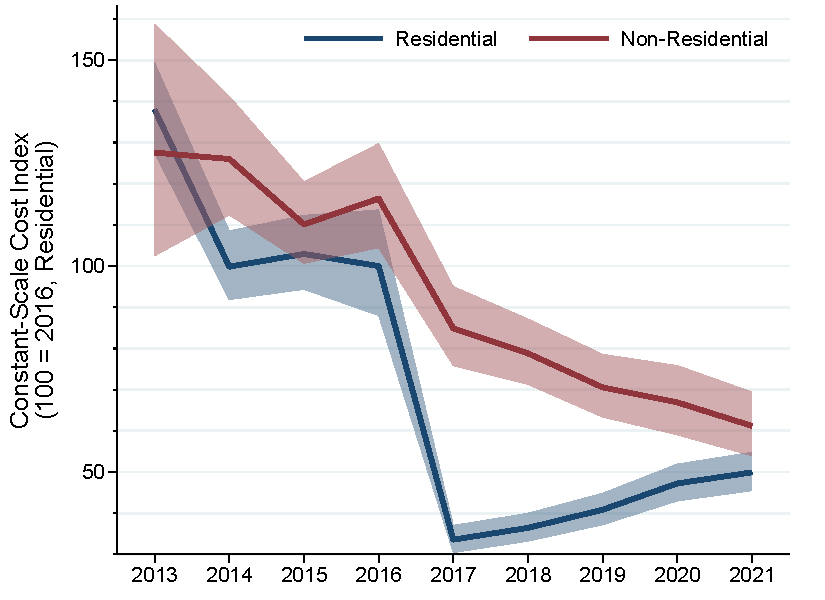
\includegraphics[width=\textwidth]{graphs/CA_SGIP/CSCI_CD.pdf}
\caption{Sector-Year Fixed Effects from Eq. \ref{eq:CD}, normalized such that $\alpha^{Res.}_{2016} = 100$}\label{fig:CSCI_CD}
\end{figure}

Figure \ref{fig:CSCI_CD} presents the estimated sector-year fixed effects of Table \ref{reg:predict_CD} in a visual format. For ease of interpretation, I have normalized all values such that the fixed effect for the residential sector in 2016 is equal to 100, following Eq. \ref{eq:CSCI}. The sector-specific trends estimated by the Cobb-Douglas model are virtually indistinguishable from those estimated by the translog model (\textit{cf.} Figure \ref{fig:CSCI_TL}).